\documentclass[12pt,a4paper]{article}

% Essential packages
\usepackage[utf8]{inputenc}
\usepackage[T1]{fontenc}
\usepackage{graphicx}
\usepackage{amsmath,amssymb}
\usepackage{booktabs}
\usepackage{color}
\usepackage{hyperref}
\usepackage{geometry}
\usepackage{float}

% Hyperlink configuration
\hypersetup{
    colorlinks=true,
    urlcolor=[rgb]{0.2,0.6,0.8},  % Light blue color for URLs
    linkcolor=black,               % Regular internal links remain black
    citecolor=black,               % Citation links remain black
}

% Page geometry
\geometry{margin=2.5cm}

% Document information
\title{Robot Arm Project Report}
\author{Luca Sartore}
\date{\today}

\begin{document}

% Title page
\begin{titlepage}
    \centering
    \vspace*{1cm}
    {\Huge\textbf{Robot Arm Project Report}\par}
    \vspace{2cm}
    {\Large\textit{Project for the introduction to robotics course}\par}
    \vspace{3cm}
    {\Large Luca Sartore\par}
    \vfill
    University of Trento
    \vspace{1cm}
\end{titlepage}

% Table of contents
\tableofcontents
\newpage

% Abstract
\section*{Abstract}
\addcontentsline{toc}{section}{Abstract}
In this report I will describe the ``Robot Arm'' project.
This project consisted of the creation of a giraffe robot with
the task of placing a microphone in front of a speaker inside a conference room.
This report will follow the assignment structure, and will therefore
have one section for each of the 8 implementation points in the 
project description that was given to me.
All the source code, as well as the original assignment, can be found in the 
GitHub repository \url{https://github.com/lucaSartore/RobotArm}


\section{Step 1 - URDF}
Building the URDF was straightforward enough.
I first focused on the structure and put together one joint at a time.
After that, I set up parameters like the limits and friction of each
joint. Then, I focused on the graphics and created a visual representation
of the robot using only basic URDF geometric tags such as ``box'' and 
``cylinder''. Finally, I inserted mass and inertia values that 
were plausible. The result can be seen in the file \href{https://github.com/lucaSartore/RobotArm/blob/master/src/robot_arm/urdf/arm.urdf}{arm.urdf}

\section{Step 2 - Forward kinematics}
The forward kinematics were computed in the ``classical'' way, using 
progressive transformation matrices for each joint, where each transformation
matrix depends on q. The code related to this part can be found in the file
\href{https://github.com/lucaSartore/RobotArm/blob/master/src/robot_arm/src/data_processing/direct_kinematics.py}{direct\_kinematics.py}.
Here we can see how the joint displacement, as well as the type of joint, are automatically
extracted from the URDF file using an XML parsing library and the Pydantic framework. Then,
a transformation matrix is computed using the function ``build\_transf\_matrix\_from\_components''.
Finally, all transformation matrices are multiplied together to obtain the transformation matrix for the end effector.

\section{Step 3 - Simulation}

For the simulation, we used the Recursive Newton-Euler Algorithm to calculate
the joint space inertia matrix ($M(q)$) as well as the non-linear effects ($h(q,\dot{q})$)
as we have seen in class. Once the forces on the joints were known, they were converted
into joint acceleration (by left-multiplying them with $M(q)^{-1}$), and 
finally, the acceleration was integrated twice to obtain joint velocity and joint position.
The code I described can be found in
\href{https://github.com/lucaSartore/RobotArm/blob/master/src/robot_arm/src/data_processing/dynamics.py}{dynamics.py}

\subsection{Damping, friction and stop force}
The process I described so far only considered the forces generated
by gravity and by the interaction between the joints. However, in this simulation,
we also included friction, damping, and stop forces (forces that are applied only when a joint
reaches the end of its allowed motion range). These were calculated
using the coefficients that were set in the URDF, making the simulation more realistic.


\subsection{Visualization}

For the visualization, the program spawns an RViz process where it constantly 
publishes the q position so that the simulation is updated in real time.
To visualize the dynamics yourself, you can run one of the following commands:
\begin{itemize}
    \item rosrun robot\_arm main.py test\_dynamics
    \item rosrun robot\_arm main.py test\_dynamics\_with\_initial\_velocity
\end{itemize}


\section{Step 4 - Trajectory}
The trajectory was planned using a fifth-degree polynomial that had the constraint of having
to reach an initial and final position, as well as requiring the
velocity and acceleration (first and second derivatives of the polynomial)
to be zero at the start and end.
The variables selected for the trajectory were the X, Y, and Z coordinates
as well as the Pitch for orientation (leaving the other two components of orientation
free).
For the orientation, I selected Euler angles as they were simple to use, and the singularity
points were really far from the operating range of the robot, making them a non-issue.
The code for the trajectory planning can be seen in
\href{https://github.com/lucaSartore/RobotArm/blob/master/src/robot_arm/src/data_processing/trajectory_planning.py}{trajectory\_planning.py}

\section{Step 5 - Cartesian controller}

The Cartesian controller implementation was straightforward. I simply used the 
desired position acceleration, as well as the tracking error and the tracking error derivative,
to calculate the desired v. I then mapped the v in task space into an acceleration in 
joint space, and used the joint space inertia matrix to map this to torque.
Finally, I linearized the system by summing the non-linear effects.
For the calculation of the non-linear effects, I first used the RENA algorithm,
but then realized that I was computing it twice (once in the dynamics and once in the controller).
Therefore, I cached the result to make the simulation slightly faster.

\begin{align*}
\textcolor{blue}{\mathbf{v}} &= \ddot{\mathbf{p}}^d + K_p (\mathbf{p}^d - \mathbf{p}) + K_d (\dot{\mathbf{p}}^d - \dot{\mathbf{p}}) \\
\textcolor{red}{\ddot{\mathbf{q}}^d} &= J^\# (\textcolor{blue}{\mathbf{v}} - \dot{J} \dot{\mathbf{q}}) \\
\mathbf{u} &= M(\mathbf{q}) \textcolor{red}{\ddot{\mathbf{q}}^d} + c(\mathbf{q}, \dot{\mathbf{q}}) + g(\mathbf{q})
\end{align*}

\section{Step 6 - PD Tuning}

To tune the PD coefficients, I started with only the KP and increased it until the tracking
error became small enough (while being careful not to increase it too much and risk creating an unstable system).
Once KP was set, I started increasing KD until the value was high enough to make the system critically damped, thus 
avoiding overshooting.

Figures \ref{fig:error_overshoot} and \ref{fig:error_not_overshoot} show charts of the absolute value of the
tracking error. In Figure \ref{fig:error_overshoot}, we can see how the error ``bounces back'' a few times
before reaching zero. In Figure \ref{fig:error_not_overshoot}, instead, we can see how the error monotonically
decreases in the second half part of the chart. This means that the system is not overshooting, thanks 
to the higher KD value.


\begin{figure}[htbp]
    \centering
    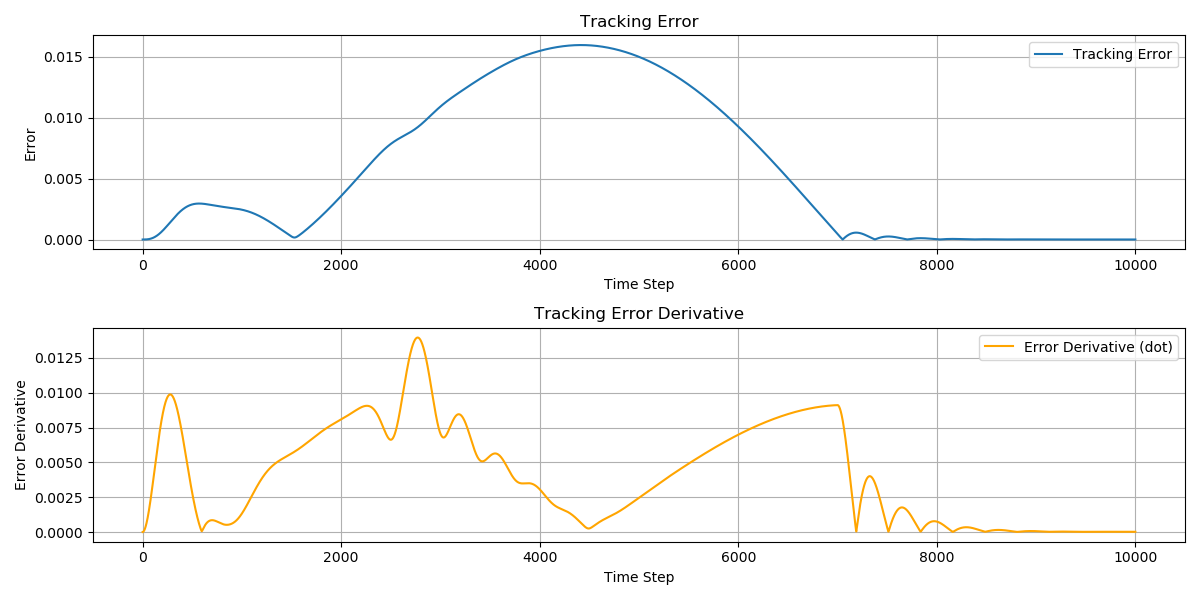
\includegraphics[width=0.7\textwidth]{images/error_chart_overshoot.png}
    \caption{The tracking error overshooting}
    \label{fig:error_overshoot}
\end{figure}


\begin{figure}[htbp]
    \centering
    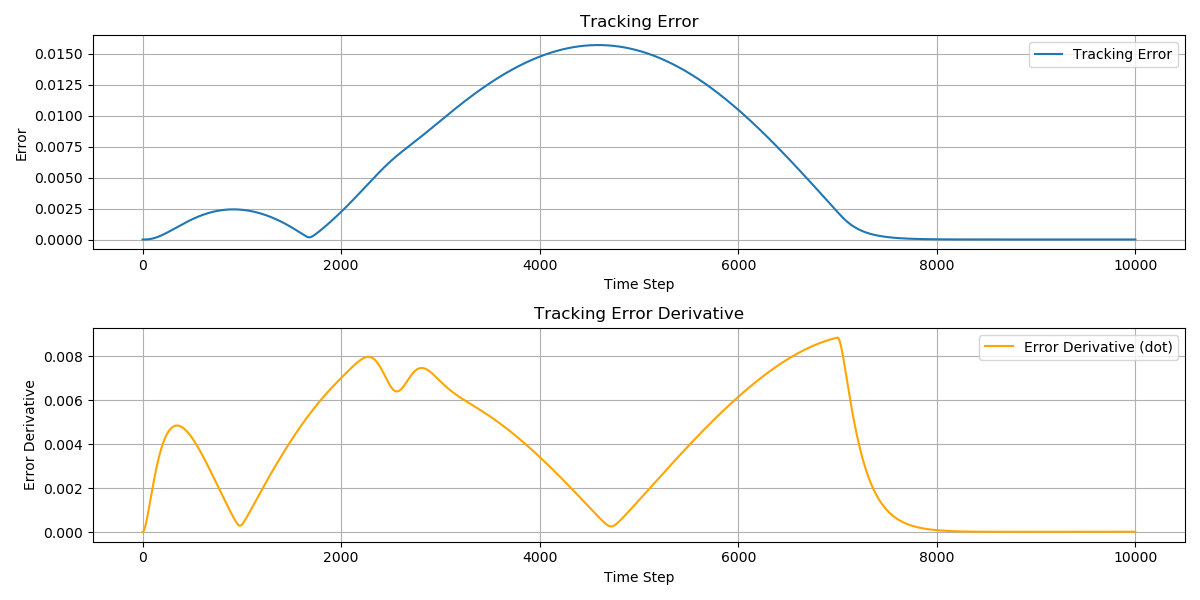
\includegraphics[width=0.7\textwidth]{images/error_chart_no_overshoot.png}
    \caption{The tracking error not overshooting}
    \label{fig:error_not_overshoot}
\end{figure}

\section{Step 7 - Postural task}
Finally, since our robot had 5 degrees of freedom, but the task controller only 
specified 4 task-space variables to control, a desired position in joint space was included in
the control loop. The final code can be seen in
\href{https://github.com/lucaSartore/RobotArm/blob/master/src/robot_arm/src/data_processing/controller.py}{controller.py}

\subsection{Selected pose and relative weights}

This postural task can be used to guide the robot towards preferred positions. For example,
while both Figure \ref{fig:undesired_pose} and \ref{fig:desired_pose} show poses that are technically
correct, the pose shown in Figure \ref{fig:undesired_pose} would be quite uncomfortable, if not dangerous,
for the people inside the conference room. In contrast, the pose shown in Figure \ref{fig:desired_pose}
is much better.

However, achieving this result was not as straightforward as one might think. I began by setting a desired
pose where all the q values were set to zero; however, I quickly realized that not all q values have the same importance.
In particular, the second q (the one controlling the pitch of the longest link) is the most important, and 
I wanted it to stay close to zero to avoid a position similar to the one in Figure \ref{fig:undesired_pose}.
However, other q values, like for example the first one (that controls the roll of the longest link),
can have almost any value, and the position will still be decent.

With this observation, I implemented a ``weighted'' postural task, where I give more weight
to the joints that I consider more important.

\begin{figure}[H]
    \centering
    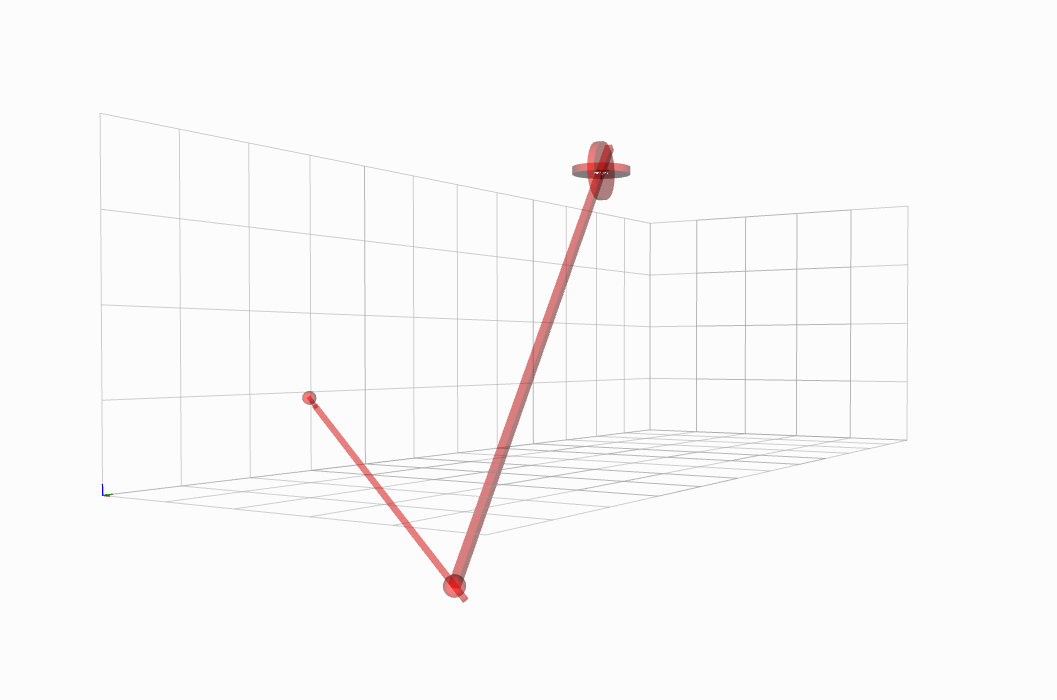
\includegraphics[width=0.7\textwidth]{images/final_position_low.png}
    \caption{An example of an undesired pose}
    \label{fig:undesired_pose}
\end{figure}


\begin{figure}[H]
    \centering
    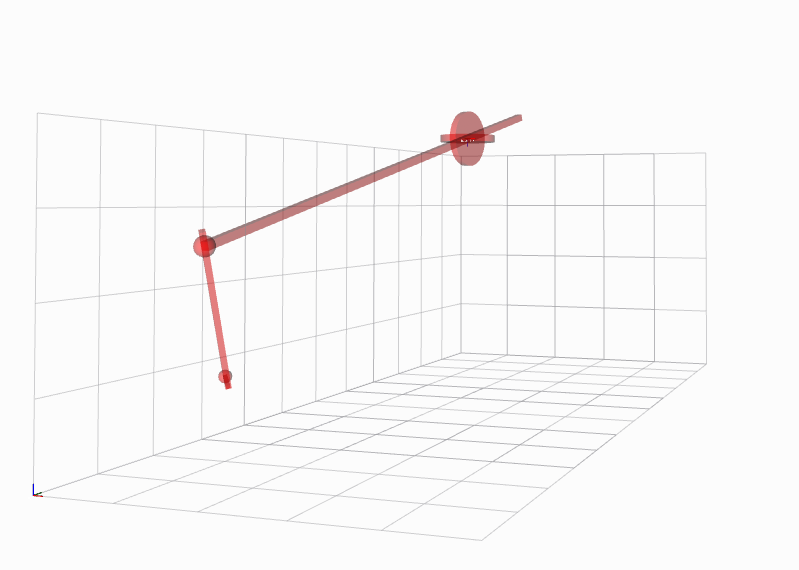
\includegraphics[width=0.7\textwidth]{images/final_positino_high.png}
    \caption{An example of a desired pose}
    \label{fig:desired_pose}
\end{figure}


\section{Step 8 - Simulation}
Finally, I put everything together and ran the simulation with the controller I designed.
The results show the robot reaching the desired position within the 7-second time limit,
and we can see that there is no overshoot.

I uploaded a video of the simulation at this URL: \url{https://www.youtube.com/watch?v=NH_AHPulZkg}. If
you prefer running the simulation yourself, you can use the command:
\begin{itemize}
    \item rosrun robot\_arm main.py
\end{itemize}



\end{document}